% HIER ALPHA-WERT ÄNDERN!
\def\alphavalue{0.15}
\def\numpoints{20}

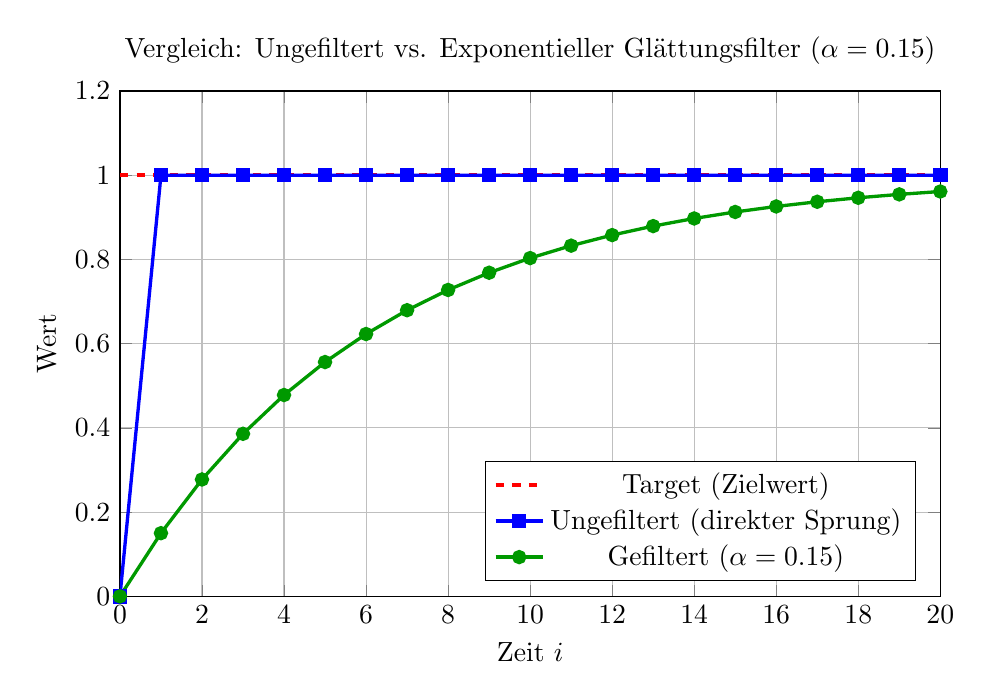
\begin{tikzpicture}
	\begin{axis}[
		width=12cm,
		height=8cm,
		xlabel={Zeit $i$},
		ylabel={Wert},
		legend pos=south east,
		grid=major,
		ymin=0,
		ymax=1.2,
		xmin=0,
		xmax=\numpoints,
		title={Vergleich: Ungefiltert vs. Exponentieller Glättungsfilter ($\alpha = \alphavalue$)}
		]
		
		% Zielwert (Target)
		\addplot[
		domain=0:\numpoints,
		samples=2,
		thick,
		dashed,
		red,
		line width=1.5pt
		] {1.0};
		\addlegendentry{Target (Zielwert)}
		
		% Ungefiltertes Signal (direkter Sprung)
		\addplot[
		mark=square*,
		blue,
		thick,
		line width=1.2pt,
		domain=0:\numpoints,
		samples=\numpoints+1
		] {x > 0 ? 1 : 0};
		\addlegendentry{Ungefiltert (direkter Sprung)}
		
		% Gefiltertes Signal - AUTOMATISCH BERECHNET!
		\addplot[
		mark=*,
		green!60!black,
		thick,
		line width=1.2pt,
		domain=0:\numpoints,
		samples=\numpoints+1
		] {x > 0 ? 1 - (1-\alphavalue)^x : 0};
		\addlegendentry{Gefiltert ($\alpha = \alphavalue$)}
		
	\end{axis}
\end{tikzpicture}